%!Tex root = bare_conf.tex
\section{Background}

\begin{figure}
\begin{subfigure}[b]{0.95\columnwidth}
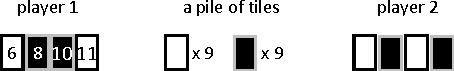
\includegraphics[width=0.95\columnwidth]{figures/DVC_procedure_1.pdf}
\caption{Initial setting}
\label{fig:DVC_procedure_1}
\end{subfigure}
\par\smallskip
\begin{subfigure}[b]{0.95\columnwidth}

\includegraphics[width=0.95\columnwidth]{figures/DVC_procedure_2.pdf}
\caption{Tile selection of palyer 1 (turn 1)}
\label{fig:DVC_procedure_2}
\end{subfigure}
\par\smallskip
\begin{subfigure}[b]{0.95\columnwidth}
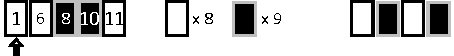
\includegraphics[width=0.95\columnwidth]{figures/DVC_procedure_3.pdf}
\caption{Tile insertion of player~1 (turn 1)}
\label{fig:DVC_procedure_3}
\end{subfigure}
\par\smallskip
\begin{subfigure}[b]{0.95\columnwidth}
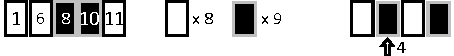
\includegraphics[width=0.95\columnwidth]{figures/DVC_procedure_4.pdf}
\caption{Tile guessing of player~1 (turn 1)}
\label{fig:DVC_procedure_4}
\end{subfigure}
\par\smallskip
\begin{subfigure}[b]{0.95\columnwidth}
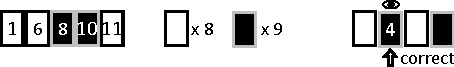
\includegraphics[width=0.95\columnwidth]{figures/DVC_procedure_5.pdf}
\caption{A case that the gussing is correct (turn 1)}
\label{fig:DVC_procedure_5}
\end{subfigure}
\par\smallskip
\begin{subfigure}[b]{0.95\columnwidth}
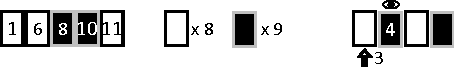
\includegraphics[width=0.95\columnwidth]{figures/DVC_procedure_6.pdf}
\caption{Consecutive tile guessing of player~1 (turn 1)}
\label{fig:DVC_procedure_6}
\end{subfigure}
\par\smallskip
\begin{subfigure}[b]{0.95\columnwidth}
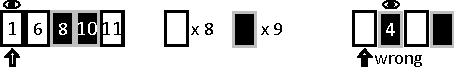
\includegraphics[width=0.95\columnwidth]{figures/DVC_procedure_7.pdf}
\caption{A case that the guessing is wrong (turn 1)}
\label{fig:DVC_procedure_7}
\end{subfigure}
\par\smallskip
\begin{subfigure}[b]{0.95\columnwidth}
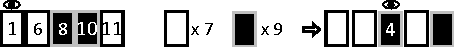
\includegraphics[width=0.95\columnwidth]{figures/DVC_procedure_8.pdf}
\caption{Tile selection of player~2 (turn 2)}
\label{fig:DVC_procedure_8}
\end{subfigure}
\par\smallskip
\begin{subfigure}[b]{0.95\columnwidth}
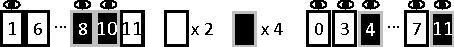
\includegraphics[width=0.95\columnwidth]{figures/DVC_procedure_9.pdf}
\caption{Winning state of player~1 (turn n)}
\label{fig:DVC_procedure_9}
\end{subfigure}
\caption{Play example of Da Vinci Code}
\end{figure}

\subsection{Da Vinci Code} \label{sec:davinci}

Da Vinci code is a board game that a player guess other player's tiles.
The game use 26 tiles which consists of two joker tiles and numbered tiles from 0 to 11. 
Half of the tiles are black and the others are white, so black 0-11 tiles, a black joker tile, white 0-11 tiles, and a white joker tile exist.
A remaining player wins when other player's all tiles are correctly guessed.

We depicts detailed procedure of Da Vinci Code with an example for clarity.
At first, all the tiles are placed on the table so that all players could not see the tiles' number.
Each player chooses four tiles form the pile and arranges them in ascending order with the smallest number on the left~(\cref{fig:DVC_procedure_1}).
A player could not see other player's tile numbers.
A turn consists of two phases.
Firstly, a player picks up a tile from the pile~(\cref{fig:DVC_procedure_2}) and inserts the tile into the right position~(\cref{fig:DVC_procedure_3}).
Secondly, the player tries to guess the opponent's tiles.
In the example, player~1 guessed the player~2's the first black tile is 4~(\cref{fig:DVC_procedure_4}).
If the tile has the same number, the opponent player must open (reveal) the tile~(\cref{fig:DVC_procedure_5}).
In the case of correct guessing, the player have a chance to guess one more tile.
In the example, we considered that the player decided to guess one more tile~(\cref{fig:DVC_procedure_6}).
When the tile has the different number, the player must open (reveal) the tile the player has brought before~(\cref{fig:DVC_procedure_7}).
When the player decided to stop or made a wrong guess, the next turn is started.
In the next turn, the opponent player conducts the same two phases~(\cref{fig:DVC_procedure_8}).
When the other players' all tiles are opened, the remaining one player wins.
In the example, player~1 wins because all the player~2's tiles are opened~(\cref{fig:DVC_procedure_9}).

\subsection{Monte Carlo Tree Search} \label{sec:mcts}

MCTS is a heuristic search algorithm for making a decision.
% It is mainly used for game play.  
The focus of MCTS is on the analysis of the most successful moves, expanding the search tree based on random sampling of the search space.
The MCTS in games is based on many cases of simulations (or playout).
In each simulation, the game is played out by selecting decision at random.
The final game result of each simulation is used to weight the nodes in the game tree so that better nodes are more likely to be chosen in future simulations.


\begin{figure}
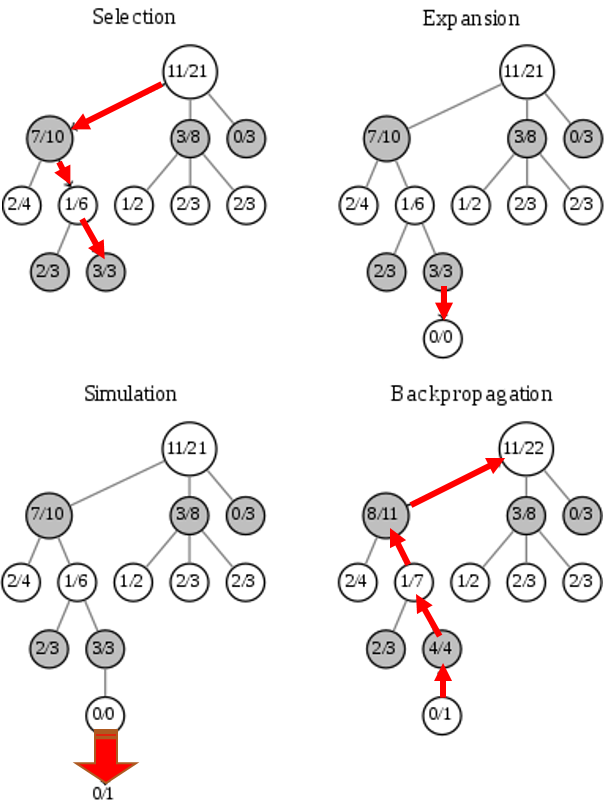
\includegraphics[width=0.95\columnwidth]{figures/MCTS_step.PNG}
\caption{Four steps of MCTS}
\label{fig:MCTS_step}
\end{figure}

MCTS consists of four steps: selection expansion, simulation, and backptropagation~(\cref{fig:MCTS_step}).
In selection, MCTS selects consecutive child nodes start from root node. 
In expansion, MCTS creates a child node of the selected node unless the selected node represents the end of game.
Simulation play a random playout from the expanded node.
Backpropagation update the result of the simulation to the nodes on the path from the expanded node to root.
After a lot of simulations, tree is expanded and represents the winning possibility when a player select the node.
Therefore, a player choose the node that have the maximum winning rate.